\begin{homeworkProblem}[Quiz 3, Pr. 2]
    \textbf{Charge Q is uniformly distributed over the volume of a
    hollow sphere of inner radius a and outer radius b, as shown. r is
    the distance from the center of the hollow part (the geometrical
    center of the structure).}

    \begin{homeworkSection}{2a}
        \textbf{Find the electric field inside the hollow part.}
        \\
        
        \begin{figure}[t]
            \centering
            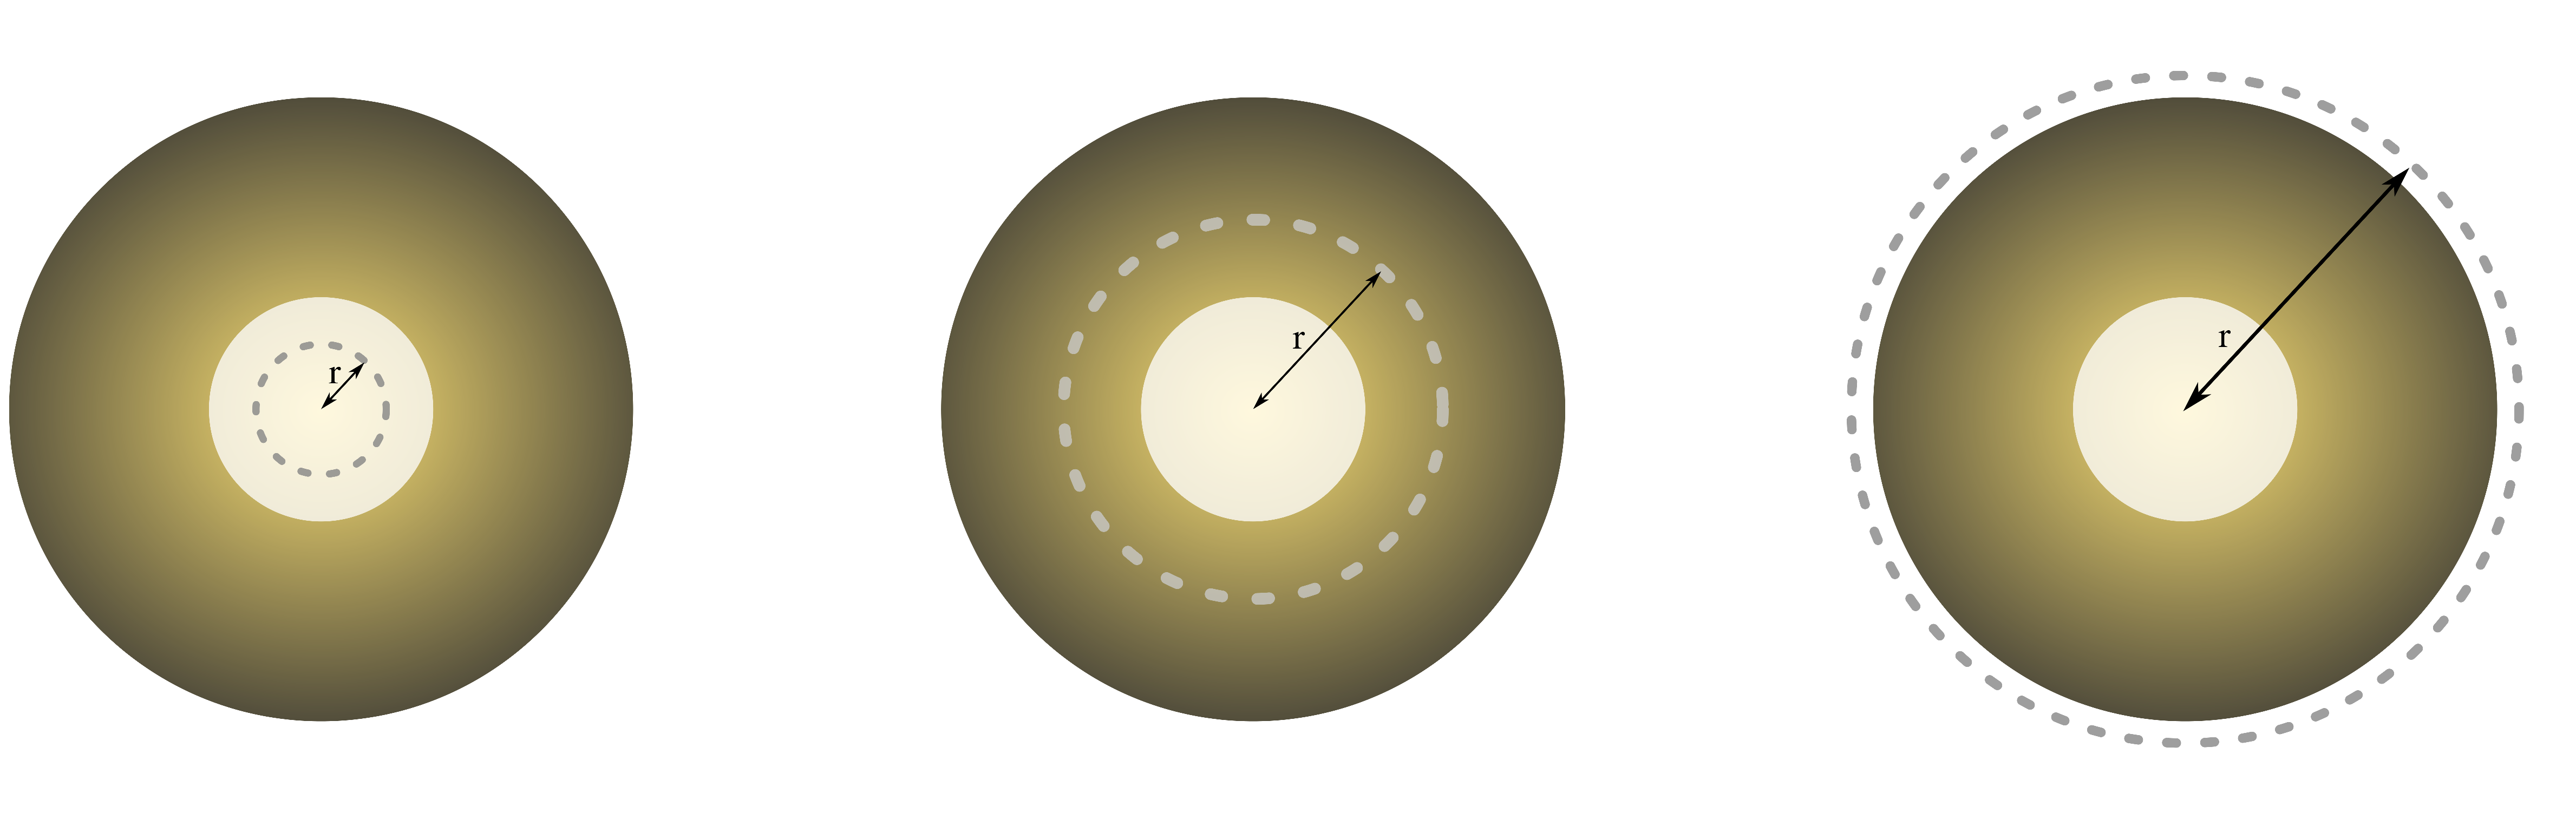
\includegraphics[width=.75\textwidth]{./img/gaussianspheres.eps}
            \caption{Hollow, charged sphere with Gaussian spheres
            located within the hollow (left), within the charged region
            (right) and encompassing all of the charge in the sphere
            (right)}
            \label{fig:gaussianspheres.eps}
        \end{figure}

        This is a little more challenging than the previous, problems.
        Now, we are dealing with a continuous distribution of charge. In
        order to find the electric field we must use Gauss' law:
        $\oint\limits_{\text{surface}}
        \vec{E}\cdot\vec{da} = \frac{Q}{\epsilon_0}$. The way in which
        we'll use Gauss' law is we'll define a surface that takes
        advantage of the symmetry of the problem. We'll pick a surface
        whose differential area vector ($\vec{da}$) is in the same
        direction as the electric field, $\vec{E}$, for all the places
        at which we need to compute this integral. The most natural
        surface to use is a sphere.
        
        The spherical charge distribution should, through symmetry
        considerations, generate an electric field that is radially
        distributed. You can justify this by imagining rotating the
        sphere. If the sphere is perfectly symmetrical then there must
        be no way that you can tell what is ``up'' ,what is ``left'',
        etc. Thus, the electric field must be symmetric with respect to
        rotations. The only distrbution of vectors that accomplishes
        this is a radial distribution.
        
        Now, our surface, our ``Gaussian surface'', will be a sphere
        with a specified radius. In this part of the problem, we are
        only asked to compute the electric field in the region where
        $r<a$. That is, in the region where there is no electric charge.
        The way in which we'll calculate the electric field is to define
        a sphere of a certain radius ($r<a$) and we'll find out how much
        charge is enclosed inside that sphere. By relating the enclosed
        charge to the surface area of our sphere we can calculate the
        electric field. Watch:

        \begin{align}
            \label{}
            \Phi = \oint\limits_{\text{sphere}} \vec{E}\cdot\vec{da} =
            \frac{Q_{enc}}{\epsilon_0} \nonumber \\
            \oint\limits_{\text{sphere}} \vec{E}\cdot\vec{da} =
            \frac{\oint\limits_{\text{charge enclosed}}\rho dV}{\epsilon_0}
        \end{align}

        Note, that my Gaussian surface, this sphere, might enclose a
        distribution of charge. So, it's necessary for me to add up all
        the charge that might be enclosed by my sphere. That's the
        reason I have rewritten the right-hand side.

        Okay, now we can simplify the expression on the left-hand side
        of the above expression. $\vec{E}$ is, by symmetry
        considerations, directed radially outward. That is $\vec{E} =
        E(r) \hat{r}$. Now, I can also argue that by symmetry the
        magnitude of the electric field should be the same at all
        distances $r$ away from the origin. Thus, $E(r)$ is a constant
        and can be pulled out of the integral. The differential area
        element $\vec{da}$, by virtue of me having chosen a sphere as my
        Gaussian surface is $da \hat{r}$. So, it is in the same
        direction as the electric field. Thus, $\vec{E}(r) \cdot
        \vec{da} = E(r) da$, where $E(r)$ is a constant. Applying all
        these simplying results yields:

        \[
        \oint\limits_{\text{sphere}} \vec{E}\cdot\vec{da} = E(r)
        \oint\limits_{\text{sphere}} da
        \]

        The last expression is just asking for the total surface area of
        the sphere (the sum of all of the differential areas is the
        total area). Thus:
        
        \[
        E(r) \oint\limits_{\text{sphere}} da = E(r) 4\pi r^2
        \]

        Where $r<a$ is the radius of our Gaussian surface. Now, how much
        charge is enclosed by our Gaussian surface for $r<a$? Nothing!
        There is no charge for $r<a$. Thus
        $\frac{\oint\limits_{\text{charge enclosed}}\rho dV}{\epsilon_0} = $.
        Since $r \ne 0$ equation 1 (along with our simplifying
        expressions) informs us that $E(r)=0$ everywhere inside the
        hollow region (for all $r<a$). Thus, the answer to 1a is $E(r<a)
        = 0$.

    \end{homeworkSection}
    \begin{homeworkSection}{2c}
        \textbf{Solve for the electric field for outside of the sphere
        where $r>b$.}
        \\

        Okay, this part of the quiz is easier than 2b, which is why I'm
        solving it first. I will start by using equation 1, which still
        applies.
        
        \[
            \oint\limits_{\text{sphere}} \vec{E}\cdot\vec{da} =
            \frac{\oint\limits_{\text{charge enclosed}}\rho dV}{\epsilon_0}
        \]

        Okay, by the same arguments as before, I can rewrite the left
        hand side as:

        \[
            E(r)\oint\limits_{\text{sphere}} da =
            \frac{\oint\limits_{\text{charge enclosed}}\rho dV}{\epsilon_0}
        \]

        Now, though, the charge enclosed is not zero. In fact, for $r>b$
        we have enclosed all of the charge on the sphere. Can we prove
        this? Yes. Let's first consider how we would find the amount of
        enclosed charge $Q_{enc} = \oint\limits_{\text{charge enclosed
        }}\rho dV$ Well, how much charge is this? It's
        $Q = \rho * V_{\text{charged hollow sphere}}$.        What is
        the volume of the charged hollow sphere? Well, it's the volume
        of a sphere of radius $b$ minus the volume of a sphere of radius
        $a$ : $V_{\text{charged hollow sphere}} = \frac{4\pi}{3}b^3 -
        \frac{4\pi}{3}a^3$. What is $\rho$? $\rho =
        \frac{Q}{V_{\text{charged hollow sphere}}}$. It is the amount of
        charge stored per volume of the charged hollow sphere.
    
        \[
        \rho = \frac{Q}{\frac{4\pi}{3}b^3 - \frac{4\pi}{3}a^3}
        \]

        Note that this is not the same thing as:
       
        \[ \rho = \frac{Q}{\frac{4\pi}{3}(b - a)^3} \]
        
        because $(a-b)^3 \ne (a^3-b^3)$, in general. The best way to
        think about the volume (to avoid algebraic mistakes) is to
        subtract the volumes of two spheres.

        So, finally, what is the total charge enclosed by our Gaussian
        surface? Well, it's our charge density, $\rho$, times the volume
        of charge enclosed. Since our Gaussian surface is larger than
        the charged sphere, though, then $V_{\text{charged hollow
        sphere}} = \frac{4\pi}{3}b^3 - \frac{4\pi}{3}a^3$, the volume of
        the entire charged hollow sphere. And, finally, $Q_{enc} =
        \rho*V_{\text{charged hollow sphere}} = Q$, the total charge on the
        sphere.

        Okay, we already said this. It makes sense. Once our Gaussian
        surface is bigger than the charged hollow sphere then our
        Gaussian surface must enclose all of the charge. But, this mode
        of thinking will help us, later, when we try to solve 2b. Okay,
        now, $\rho$ is a constant so we can pull it out of the
        right-hand side of our expression for Gauss' law. Then, we're
        just integrating over the volume of our Gaussian surface. For a
        Gaussian surface with radius $r>b$, the Gaussian surface's
        volume is just $\frac{4\pi}{3} r^3$. Thus, our expression for
        Gauss' law can be reduced to:

        \[
            E(r) 4\pi r^2 = \frac{Q}{\epsilon_0}
        \]

        Now, $E(r) = \frac{Q}{4\pi\epsilon_0 r^2} = \frac{kQ}{r^2}$.
        This is an important result. Outside of a spherically symmetric
        charge distribution, the electric field looks like exactly that of
        a point charge located at the origin. How big is that point
        charge? Well, it's as big as the amount of charge stored in that
        spherically symmetric charge distribution. Okay, this is the
        answer for 2c. Let's tackle 2b.
        
    \end{homeworkSection}
    \begin{homeworkSection}{2b}

        Okay, we'll start with Gauss' law. I'll immediately apply the
        symmetry results to simplify the expression.

        \[
            E(r)\oint\limits_{\text{sphere}} da =
            \frac{\oint\limits_{\text{charge enclosed}}\rho dV}{\epsilon_0}
        \]

        We have the expression for $\rho$ from before.
        \[ \rho = \frac{Q}{\frac{4\pi}{3}(b^3- a^3)} \]

        Now, $\rho$ is a constant (uniform charge distribution), so I
        can pull this out of the integral. The integral on the left-hand
        side over $da$ is just the area of our Gaussian surface $\oint
        da = A = 4\pi r^2$, as usual. The most difficult thing in this
        problem is the integral over $dV$ in the right-hand side. This
        is not the volume of our Gaussian surface! We are trying to
        calculate the amount of enclosed charge. Thus, this volume
        should be the volume of the enclosed charge. At a distance $r$
        from the center, the amount of charge I have enclosed is

        \[
        V_{\text{charge enclosed}} = \frac{4\pi}{3}r^3 -
        \frac{4\pi}{3}a^3
        \]

        It's exactly the volume of my Gaussian surface \textbf{minus the
        volume of my Gaussian surface in which there is no charge}. This
        is the center of the hollow sphere. Substituting this yields:

        \[
        E(r)4\pi r^2  = \frac{1}{\epsilon_0} \bigg(
        \frac{Q}{\frac{4\pi}{3}b^3 - \frac{4\pi}{3}a^3}\bigg) \bigg( \frac{4\pi}{3}
        r^3 -\frac{4\pi}{3}a^3 \bigg)
        \]

        After a little algebra this can be rewritten as:

        \[
        E(r) = \frac{Q}{4\pi \epsilon_0 r^2} \frac{r^3-a^3}{b^3-a^3}
        \]

        This is the answer for problem 2b.
    \end{homeworkSection}
    \begin{homeworkSection}{2d}
        \textbf{Solve for the electric field at the outer surface where
        $r=b$.}
        \\

        Now, this problem is very simple. We just have to plug in $r=b$
        into our expressions for $E(r)$ from either part b or or part c.
        How come we can use either expression? Well, the electric field
        outside the sphere, for all $r>b$, is given by the answer in 2c.
        The electric field inside the sphere, for $a<r<b$, is given in
        2b. So, taking the limit as $r\rightarrow b$ both expressions
        should yield the same thing, if a limit exists. And, this is a
        fairly simple situation, that could be constructed fairly
        easily, so we hope a limit exists. It's easiest to plug $r=b$
        into the answer we got in 2c, but we could just as well plug it
        into 2b. If we do this, we obtain:

        \[
        E(b) = \frac{kQ}{b^2}
        \]
    \end{homeworkSection}
\end{homeworkProblem}
